\subsection{Screen buffer}

Instead of constantly calculating how the screen looks, we have a buffer that keeps a copy of the screen in an array. This enables os to do calculations easier and also only update parts of the screen as needed. To save space it keeps 8 pixels state per uint8\_t in it's internal buffer.

\subsubsection{Setup}

The setup of this buffer is performed automaticlly via templates on compiletime. The only requirements there are to the Display is the following variables and method. This enables the buffer to be used with other Display's without the need to change in the implementation.

\begin{itemize}
\item SetAddress
\item Write
\item rows
\item columns
\item addressing\_static
\item addressing\_vertical
\item current\_addressing\_vertical (only needed if addressing\_static is false)
\end{itemize}

The two first methods are used to set the row and column to where we want to write on the Display and to actually write there.

The next two are used to create a correctly sized array on compiletime and eliminating any dynamic allocation.

As many displays can either work in vertical mode or horizontal mode (see figure~\ref{fig:array_horizontal} and~\ref{fig:array_vertical} ) - or some dynamicly change between the two modes, the last two/three variables are used to optimize the communication to the Display.

\begin{figure}
\centering
\begin{minipage}{.5\textwidth}
  \centering
  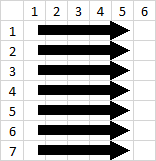
\includegraphics[width=.4\textwidth]{implementation/array_horizontal}
  \caption{Horizontal Addressed Display}
  \label{fig:array_horizontal}
\end{minipage}%
\begin{minipage}{.5\textwidth}
  \centering
  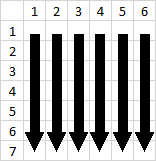
\includegraphics[width=.4\textwidth]{implementation/array_vertical}
  \caption{Vertical Addressed Display}
  \label{fig:array_vertical}
\end{minipage}
\end{figure}


If the Display can shift between vertical and horizontal mode, then we need a runtime check on the current\_addressing\_vertical to be sure we are writing the correct way (see Listing~\ref{lst:dynamic_mode}). Now if the Display only works in one direction, then there's no need to have this runtime check. So if the addressing\_static is true on compiletime, only the correct direction is compiled into the binary and used directly (see Listing~\ref{lst:static_vertical}).

\noindent\begin{minipage}[t]{.45\textwidth}
\begin{lstlisting}[caption={Dynamic Mode},label={lst:dynamic_mode},frame=tlrb, language=C++]{Name}
template<typename Q = DISPLAY>
typename enable_if<!Q::addressing_static, void>::type
update(Point point, uint8_t width, uint8_t height) {
    if (display->current_addressing_vertical) {
  	    update_vertical(point, width, height);
  	} else {
  			update_horizontal(point, width, height);
  	}
}
\end{lstlisting}
\end{minipage}\hfill
\begin{minipage}[t]{.45\textwidth}
\begin{lstlisting}[caption={Static Vertical Mode},label={lst:static_vertical},frame=tlrb, language=C++]{Name}
template<typename Q = DISPLAY>
typename enable_if<Q::addressing_static && Q::addressing_vertical_mode, void>::type
update(Point point, uint8_t width, uint8_t height) {
    update_vertical(point, width, height);
}
\end{lstlisting}
\end{minipage}

\subsubsection{Usage}

The user of the buffer should not in general worry about how the data is stored in the 8 pixel's per uint8\_t. The only funtion that allows the user to access the array directly is the set\_data, which is used for text that matches the 8 bit height.

The rest of the function uses pixel x,y coordinates. The two main functions are the draw\_square and clear\_square as most other figures can be made with these. They calculate / recalculate the dimension given, to make sure only the part inside the screen is added. It also does the hard merging part of already existing data and the new data, when they share the same uint8\_t.
